\documentclass{bioinfo}
\bibliographystyle{natbib}
%\bibliographystyle{achemnat}
%\bibliographystyle{plainnat}
%\bibliographystyle{abbrv}
%\bibliographystyle{bioinformatics}

\copyrightyear{2011}
\pubyear{2011}

\begin{document}
\firstpage{1}

\title[Knime4Bio]{Knime4Bio: a set of custom nodes for the interpretation of Next Generation Sequencing data with KNIME.}
\author[Pierre Lindenbaum \textit{et~al}]{Pierre Lindenbaum\,$^{1}$, Solena Le Scouarnec\,$^{2}$,  Vincent Portero\,$^{1}$ and Richard Redon\,$^{1,}$\footnote{to whom correspondence should be addressed}}
\address{$^{1}$Institut du thorax, Inserm UMR 915, Centre Hospitalier Universitaire de Nantes, 44000 Nantes, France.\\
$^{2}$The Wellcome Trust Sanger Institute, Hinxton, Cambridge CB10 1SA, UK.}

\history{Received on XXXXX; revised on XXXXX; accepted on XXXXX}

\editor{Associate Editor: XXXXXXX}

\maketitle

\begin{abstract}

\section{Summary:}
Analysing large amounts of data generated by next-generation sequencing (NGS) technologies is difficult for researchers or clinicians without computational skills. They are often compelled to delegate this task to computer biologists working with command line utilities. The availability of easy-to-use tools will become essential with the generalisation of NGS in research and diagnosis. It will enable investigators to handle much more of the analysis. Here, we describe Knime4Bio, a set of custom nodes for the KNIME (The Konstanz Information Miner) interactive graphical workbench, for the interpretation of large biological datasets. We demonstrate that this tool can be utilised to quickly retrieve previously published scientific findings.

\section{Availability:}
\href{http://code.google.com/p/knime4bio/}{http://code.google.com/p/knime4bio/}.

\section{Contact:} \href{mailto:richard.redon@univ-nantes.fr}{richard.redon@univ-nantes.fr}
\end{abstract}

\section{Introduction}

Next-generation sequencing (NGS) technologies have led to an explosion of the amount of data to be analysed. As an example, a VCF~\citep{pmid21653522} file (Variant Call Format - a standard specification for storing genomic variations in a text file) produced by the 1000 Genomes Project contains about 25 million Single Nucleotide Variants (SNV)\footnote{\href{ftp://ftp-trace.ncbi.nih.gov/1000genomes/ftp/release/20100804/ALL.2of4intersection.20100804.sites.vcf.gz}{http://tinyurl.com/ALL2of4intersection} . Retrieved Sept. 2011.}, making it difficult to extract relevant information using spreadsheet programs. Whilst computer biologists are used to invoke common command line tools - such as Perl and R - when analysing those data through Unix pipelines, scientific investigators generally lack the technical skills necessary to handle these tools and need to delegate data manipulation to a third-party. 

Scientific workflow and data integration platforms aim to make those tasks more accessible to those research scientists. These tools are modular environments enabling an easy visual assembly and an interactive execution of an analysis pipeline (typically a directed graph) where a node defines a task to be executed on input data and an edge between two nodes represents a data flow. These applications provide an intuitive framework that can be used by the scientists themselves for building complex analyses. They allow data reproducibility and workflows sharing.

Galaxy \citep{pmid21531983}, Cyrille2~\citep{pmid18269742} and Mobyle~\citep{pmid19689959} are three web-based workflow engines that users have to install locally if computational needs on data sets are very large, or if absolute security is required. Alternatively, softwares such as the KNIME~\citep{knimeref} workbench or Taverna~\citep{pmid16845108}  run on the users' desktop and can interact with local resources. Taverna focuses on web services and may require a large number of nodes even for a simple task. In contrast KNIME provides the ability to modify the nodes without having to re-run the whole analysis. We have choosen this latest tool to develop Knime4Bio, a set of new nodes mostly dedicated to the filtering and manipulation of VCF files. Although many standard nodes provided by KNIME can be used to perform such analysis, our nodes add new functionalities, some of which are described below.

\section{Implementation}

The java API for KNIME was used to write the new nodes. They were deployed and documented using some dedicated XML descriptors.
\\
A typical workflow for analysing exome sequencing data starts by loading VCF files into the working environment. The data contained in the INFO or the SAMPLE columns are extracted and the next task consists in annotating SNVs and/or indels. A node predicts the consequence of variations at the transcript/protein level. For each variant, genomic sequences of overlapping transcripts are retrieved from the UCSC knownGene database~\citep{pmid16500937} to identify variants leading to premature stop codons, non-synonymous variants, and variants likely to affect splicing.  Some nodes have been designed to find the intersection between the variants in the VCF file and a various source of annotated genomic regions, which can be: a local BED file, a remote URL, a mysql table, a file indexed with tabix~\citep{pmid21208982}, a BigBed or a BigWig file~\citep{pmid20639541}. Other nodes are able to incorporate data from other databases: dbSNFRP~\citep{pmid21520341}, dbSNP, Entrez Gene, PubMed, the EMBL STRING database, Uniprot, Reactome, and GeneOntology~\citep{pmid17098935}, MediaWiki, or to export the data to SIFT~\citep{pmid11337480}, Polyphen2~\citep{pmid20354512}, BED, or MediaWiki formats. After being annotated, some SNVs (e.g. intronic) can be excluded from the dataset and the remaining data are rearranged by grouping the variants per sample or per gene as a pivot table. Some visualisation tools have also been implemented: the Picard API~\citep{pmid19505943} or the IGV browser~\citep{pmid21221095} can be used visualise the short reads overlapping a variation.
\\
As a proof of concept we tested our nodes to analyse the exomes of six patients from a previously published study~\citep{pmid21378989} related to the Hajdu Cheney syndrome (Fig.~\ref{fig:x1}). For this purpose, short reads were mapped to the human genome reference sequence using BWA~\citep{pmid20080505} and variants were called using SAMtools mpileup~\citep{pmid19505943}. Homozygous variants, known SNPs (from dbSNP), and poor-quality variants were discarded, and only non-synonymous and variants introducing premature stop codons were considered. , On a RedHat server (64bits, 4 processors, 2GB of RAM) our KNIME pipeline generated a list of 6 genes in 45 minutes: \href{http://www.ncbi.nlm.nih.gov/gene/9620}{\textit{CELSR1}},  \href{http://www.ncbi.nlm.nih.gov/gene/1284}{\textit{COL4A2}}, \href{http://www.ncbi.nlm.nih.gov/gene/64110}{\textit{MAGEF1}}, \href{http://www.ncbi.nlm.nih.gov/gene/51168}{\textit{MYO15A}}, \href{http://www.ncbi.nlm.nih.gov/gene/84905}{\textit{ZNF341}} and more importantly \href{http://www.ncbi.nlm.nih.gov/gene/4853}{\textit{NOTCH2}} the expected candidate gene\footnote{The workflow was posted on myexperiment.org at: \href{http://www.myexperiment.org/workflows/2320.html}{www.myexperiment.org/workflows/2320}}.

\begin{figure}[!tpb]%figure1
\centerline{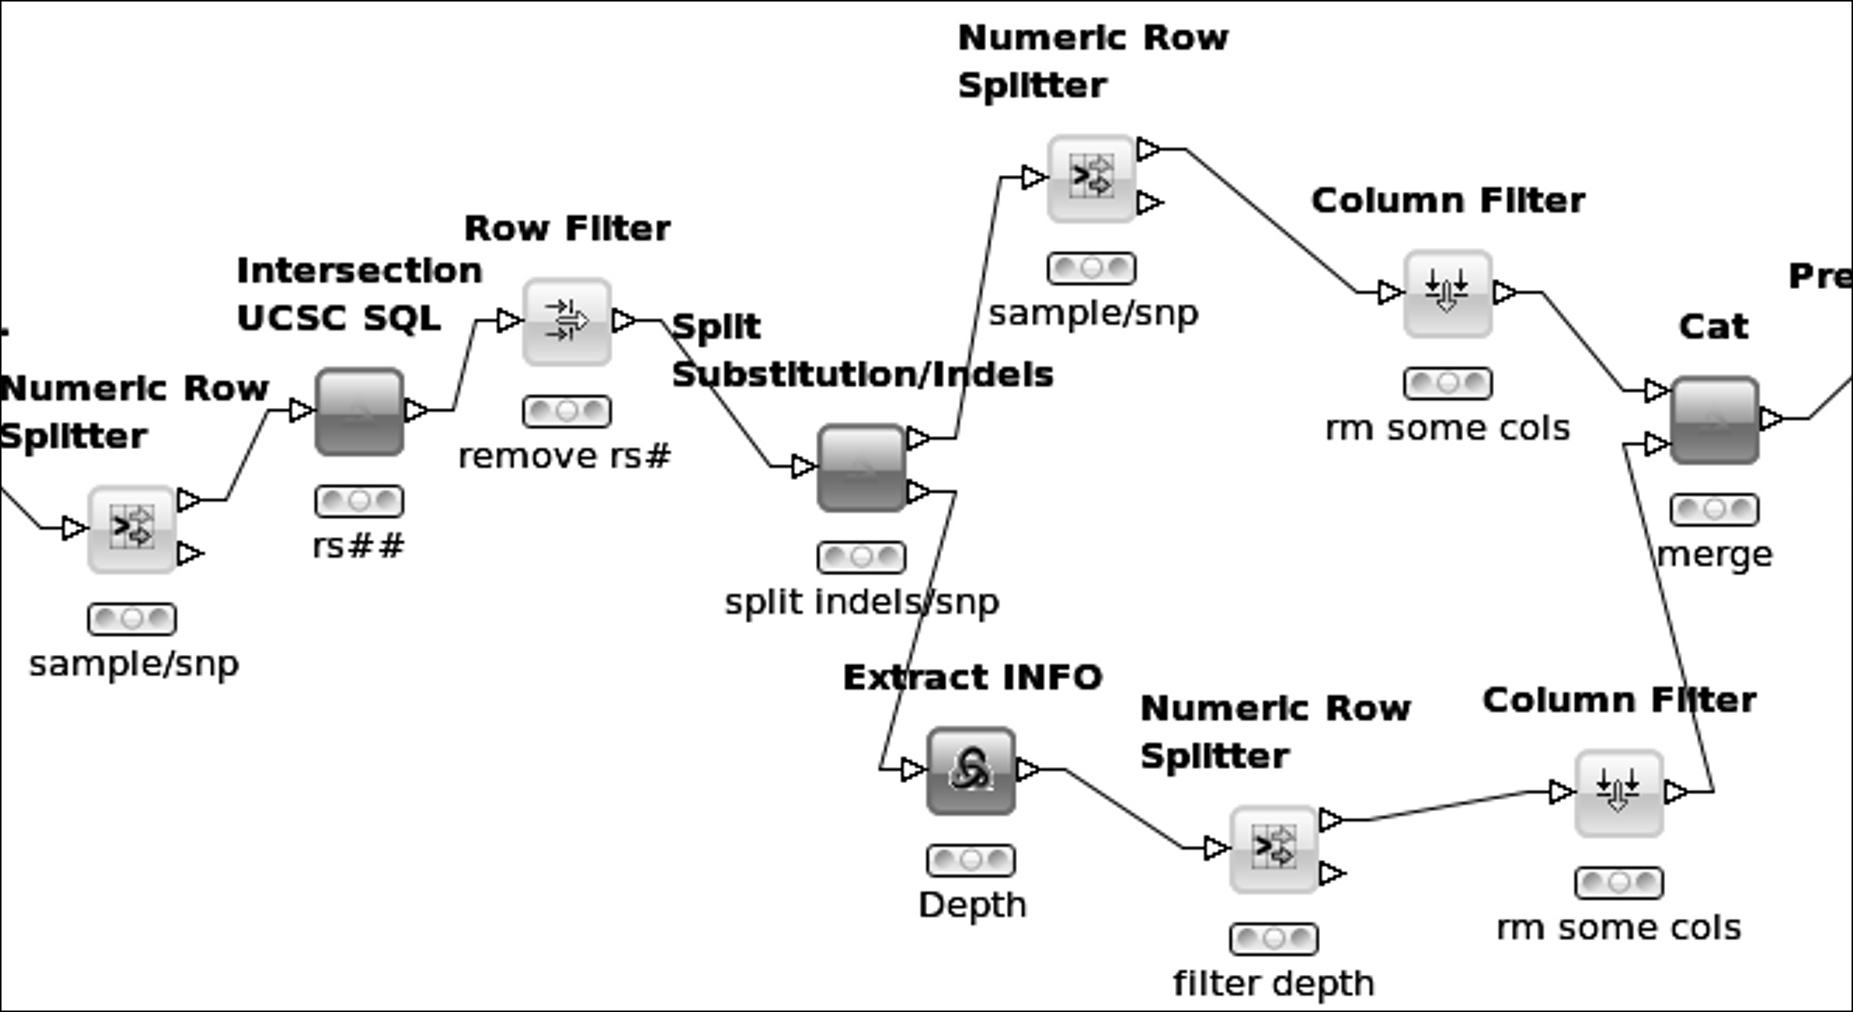
\includegraphics{fig01.eps}}
\caption{Screenshot of a Knime4Bio workflow for the NOTCH2 analysis.}\label{fig:x1}
\end{figure}

\section{Discussion}
In practical terms, a computer biologist was close to our users to help them with the construction of a workflow. After this short tutorial, they were able to quickly play with the interface, add some nodes and modify the parameters without any further assistance but the suggestion or the configuration of some specific nodes (for example those who require a snippet of java code).  At the time of writing, Knime4Bio contains 55 new nodes. We believe Knime4Bio is an efficient interactive tool for next-generation sequencing analysis.

\section*{Acknowledgements}
We want to thank the  \href{http://biostar.stackexchange.com/}{Biostar community} for its help, Jim Robinson and his team for the \href{http://code.google.com/p/bigwig/}{BigWig java API}, and Dr Cedric Le Caignec for the \textit{NOTCH2} data.

\paragraph{Funding\textcolon} This work was supported by the Inserm, the "Centre Hospitalier Universitaire" of Nantes, the "F\'{e}d\'{e}ration Fran\c{c}aise de Cardiologie" (FFC) and the "Fondation pour la Recherche M\'{e}dicale" (FRM). Solena Le Scouarnec is supported by the Wellcome Trust (Grant n° WT077008).

\paragraph{Note\textcolon} During the reviewing process of this article another solution based on KNIME but focusing on FASTQ data files was published by Jagla \textit{et~al}~\citep{pmid21873641}.
\\

\bibliography{knime}

\end{document}
